\documentclass{article}
\usepackage{amsmath}
\usepackage{tikz}
% Title
\author{Daniel Bustos}
\date{30/04/2024}
\title{Interseccion Maxima}

\begin{document}
\maketitle

Sea $G = (E,V)$ un grafo conexo. Queremos ver que todo par de caminos simples de longitud máxima de $G$ tienen un vértice en común.

Supongamos dos caminos $P = v_1, v_2, v_3, \ldots, v_n$ y $Q = w_1, w_2, w_3, \ldots, w_n$ de misma longitud tal que todos sus vértices son distintos entre sí.

Supongamos que $|P| = |Q|$ con esta siendo la longitud máxima posible de camino simple en $G$.

Observemos que como $G$ es conexo, se cumple que debe existir un camino entre todos los vértices. Este no necesariamente es simple. Pero podemos arreglar esto más adelante.

Tomemos el camino $C$, que va desde $v_1$ hasta $w_n$, este es de la forma 

\[ C = v_1, \ldots, v_i, \ldots, w_j, \ldots, w_n \]

con $v_i'$ el punto que se conecta a $w_j$ . LLamemos INT a los nodos intermedios en la conexion:


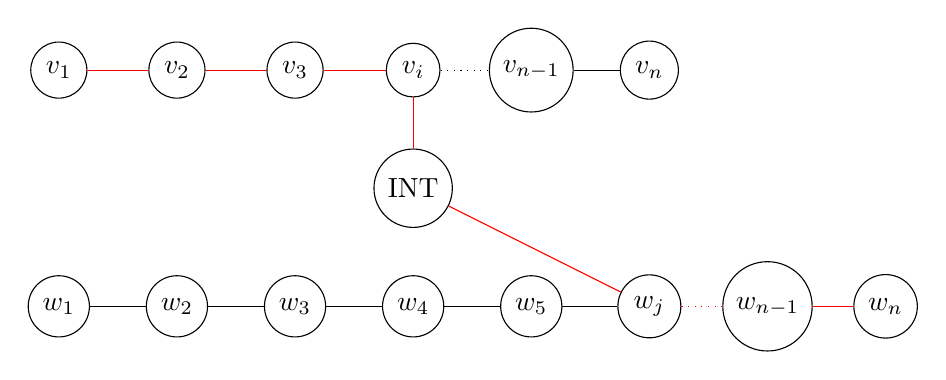
\begin{tikzpicture}
    % Nodes for the v_i part
    \node[circle,draw] (v1) at (0,0) {$v_1$};
    \node[circle,draw] (v2) at (1.5,0) {$v_2$};
    \node[circle,draw] (v3) at (3,0) {$v_3$};
    \node[circle,draw] (vi) at (4.5,0) {$v_i$};
    \node[circle,draw] (vn1) at (6,0) {$v_{n-1}$};
    \node[circle,draw] (vn) at (7.5,0) {$v_n$};
    \node[circle,draw] (INT) at (4.5,-1.5) {INT};

    % Nodes for the w_j part
    \node[circle,draw] (w1) at (0,-3) {$w_1$};
    \node[circle,draw] (w2) at (1.5,-3) {$w_2$};
    \node[circle,draw] (w3) at (3,-3) {$w_3$};
    \node[circle,draw] (w4) at (4.5,-3) {$w_4$};
    \node[circle,draw] (w5) at (6,-3) {$w_5$};
    \node[circle,draw] (wj) at (7.5,-3) {$w_j$};
    \node[circle,draw] (wn1) at (9,-3) {$w_{n-1}$};
    \node[circle,draw] (wn) at (10.5,-3) {$w_n$};

    % Edges for the v_i part
    \draw[red] (v1) -- (v2);
    \draw[red] (v2) -- (v3);
    \draw[red] (v3) -- (vi);
    \draw[dotted] (vi) -- (vn1);
    \draw (vn1) -- (vn);

    % Edges for the w_j part
    \draw (w1) -- (w2);
    \draw (w2) -- (w3);
    \draw (w3) -- (w4);
    \draw (w4) -- (w5);
    \draw (w5) -- (wj);
    \draw[dotted][red] (wj) -- (wn1);    
    \draw[red](wn1) -- (wn);

    % Connection between v_i and INT
    \draw[red] (vi) -- (INT);

    % Connection between INT and w_j
    \draw[red] (INT) -- (wj);
\end{tikzpicture}





¿Cuánto mide $C$? Llamemos a \#INT la cantidad de vértices intermedios, que pueden ser 0 o más. Entonces, usando que $|P| = |Q| = n$:

Ya que la longitud de los caminos es la misma. Sabemos que:  

\[ i + (n - j) + 1 = n + 1 \]

Luego la longitud total de $C$ es:

\[ |C| = n + 1 + \#INT \]

Entonces $|C| > n = |P| = |Q|$ ya que  $ \#INT \ge 0$\\ 
¿Es $C$ simple? Si! P y Q no tienen elementos en común y cualquier elemento intermedio no pertenece a ninguno de los dos. Entonces es simple.

Observemos que  construimos un nuevo camino mayor a P y Q simple, pero P y Q eran máximos. ¡Absurdo!

Por lo tanto, el absurdo provino de suponer que P y Q no tenían ningún vértice en común. Así que vale lo que queríamos probar.

\end{document}
